%Параметры страницы для большей схожести с веб-версией
\documentclass[12pt]{article}
\usepackage[total={170mm,230mm}]{geometry}

\usepackage{cmap}
%\usepackage{hyperref}
\usepackage[utf8]{inputenc}
\usepackage[T2A]{fontenc}
\usepackage[russian]{babel}

\usepackage{graphicx}
\usepackage{xcolor}
\usepackage{amssymb}
\usepackage{amsfonts}
\usepackage{amsmath}
\usepackage{amsthm}
\usepackage{physics}
\usepackage{wrapfig}
\usepackage{cancel}
\usepackage{pdfpages}
\usepackage{hyperref}
\newtheorem{definition}{Опредление}[section]
\newtheorem{theorem}{Теорема}[section]
\newtheorem{axiom}{Аксиома}[section]

\usepackage{pgfplots}
\pgfplotsset{width=7cm,compat=newest}

\usepackage{amsmath}
\DeclareMathOperator\arctanh{arctanh}

\usepackage{amsmath}
\DeclareMathOperator\arccosh{arccosh}

\usepackage{amsmath}
\DeclareMathOperator\const{const}

\title{Ряды с неотрицательными слагаемыми}
\author{Алексей Савватеев \and Александр Тонис}

\begin{document}
\maketitle
\begin{abstract}
В данной лекции подробно рассмотрены ряды с неотрицательными слагаемыми, дано их опредление, приведены определения сходящегося и расходящегося рядов, затронута аксиома полноты, изложены такие методы суммирования рядов и оценки их сумм, как метод перегруппировки слагаемых, интегральный признак, признак сходимости Даламбера и признак Коши. Почти каждая затронутая тема подкреплена примерами.
\par
Конспектировал Александр Козлов. 
\end{abstract}
\newpage
\tableofcontents
\newpage
\section{Геометрическая прогрессия}
\subsection{Ряды}
Дадим важное вводное определение.
\begin{definition}
\emph{Ряд}~\----~это бесконечная сумма слагаемых:
\begin{equation}
    a_1 + a_2 + \ldots + a_n + \ldots
\end{equation}
\end{definition}
Пока что будем рассматривать лишь ряды с положительными слагаемыми. Следующий ряд называют \emph{гармоническим}:
\begin{equation}\label{eq:1}
    1 + \dfrac{1}{2} + \dfrac13 + \dfrac14 + \dfrac15 + \ldots
\end{equation}
Он представляет из себя сумму чисел, обратных натуральным. Так же рассмотрим ряд:
\begin{equation}\label{eq:2}
    1 + \dfrac{1}{2} + \dfrac14 + \dfrac18 + \dfrac{1}{16} + \ldots
\end{equation}
Он характерен тем, что каждый следующий член ряда вдвое меньше предыдущего. То есть набор элементов ряда представляет собой \emph{геометрическую прогрессию} со знаменателем $1/2$.
\subsection{Выводы о сумме рядов}
Таким образом мы имеем дело с двумя бесконечными суммами. Оказывается, что ряду (\ref{eq:2}) отвечает определённое значение его суммы, в то время как ряду (\ref{eq:1}) определённое значение суммы не отвечает. Проиллюстрируем данный факт. Обратимся сперва к ряду (\ref{eq:2}). Начнём считать его \emph{частичне суммы} (так называют суммы конечного числа первых элементов ряда). Сумма первых двух элементов ряда представима в виде
\begin{equation}
    1 + \dfrac12 = 2 - \dfrac12.
\end{equation}
Сумму первых трёх членов ряда можно записать следующим образом:
\begin{equation}
    1 + \dfrac12 + \dfrac14 = 2 - \dfrac14.
\end{equation}
Сумма первых четырёх элементов даёт
\begin{equation}
    1 + \dfrac12 + \dfrac14 + \dfrac18 = 2 - \dfrac18.
\end{equation}
Можно заметить, что каждый раз прибавляется половина оставшегося расстояния до точки $2$ (см. рис. \ref{fig:1}). То есть частичная сумма одного элемента удалена от $2$ на $1$, частичная сумма двух элементов удалена от $2$ на $1/2$ и так далее. 
\begin{figure}[ht]
    \centering
    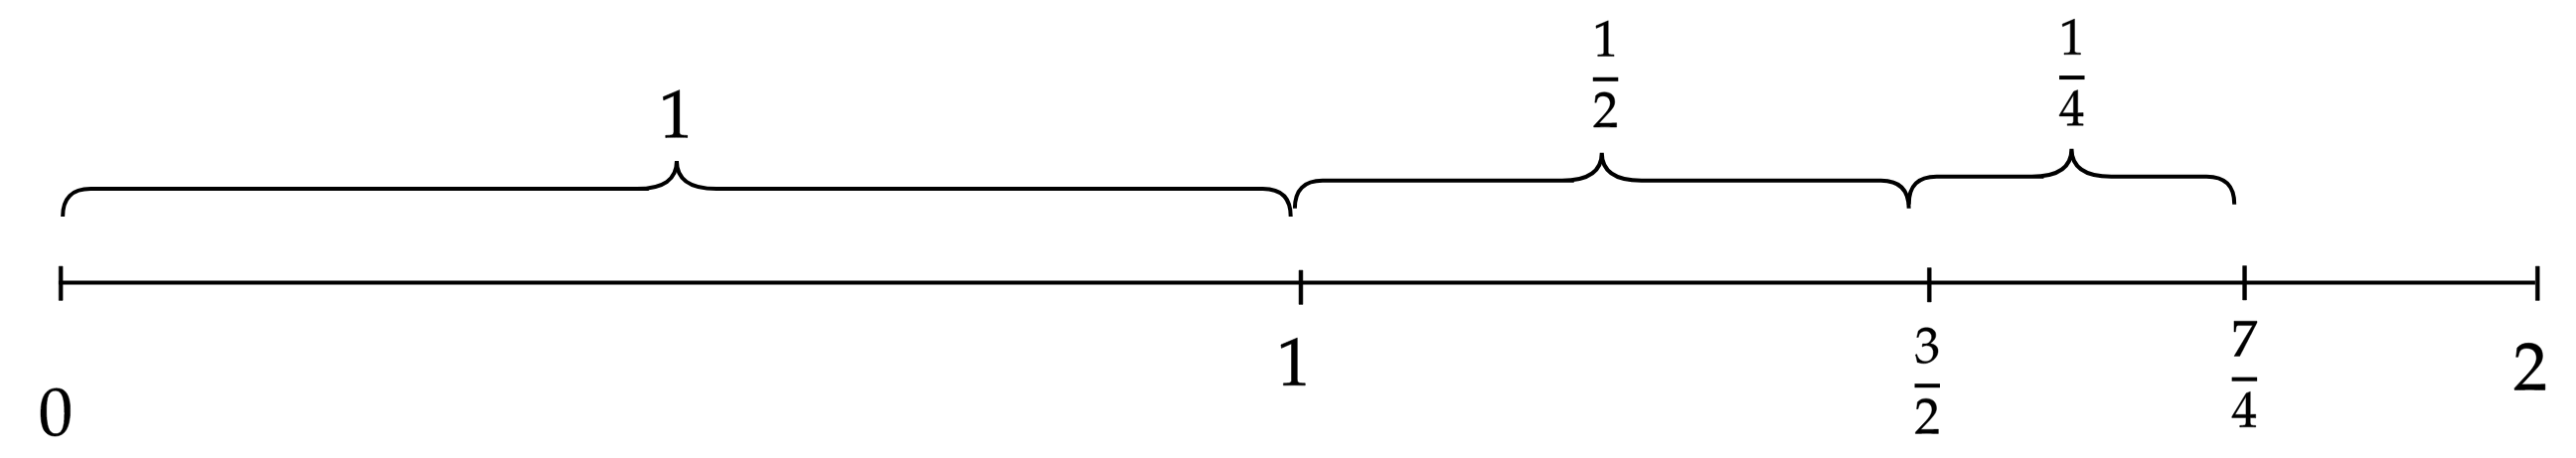
\includegraphics[width = 1\textwidth]{fig1.png}
    \caption{Графическое представление последовательности частичных сумм ряда (\ref{eq:2}).}
    \label{fig:1}
\end{figure}
Удаётся доказать методом математической индукции утверждение, что частичная сумма $n$ членов ряда удалена от $2$ на $1/{2^{n-1}}$. Тогда выходит, что \emph{сколь угодно большое количество членов ряда не просуммируй~\----~всё равно их сумма будет меньше $2$}. С другой строны, с увеличением $n$ частичная сумма $n$ членов ряда всё ближе и ближе подходит к $2$. Это явление называют \emph{неограниченным приближением суммы ряда к $2$}.
\subsection{Кванторы и определение суммы ряда}
Для большей лаконичности подобные выводы принято записывать с помощью специальных математических символов~\----~\emph{кванторов}. С помощью символа $\forall$ обозначают "для любого"{}, а под символом $\exists$ понимают "найдётся"{} или "существует"{}. Введём так же символ ":"{}, им будем обозначать\footnote{Иногда вместо двоеточия используют вертикальную черту} слова "такое(\--ие), что"{}. Тогда с помощью введённых символов можно оформить полученные выше выводы о сумме ряда (\ref{eq:2}) следующим образом:
\begin{equation}\label{eq:6}
    \forall \varepsilon > 0 \quad \exists n: \quad 2 > 1 + \dfrac{1}{2} + \dfrac14 + \dfrac18 + \dfrac{1}{16} + \ldots + \dfrac1{2^{n-1}} > 2 - \varepsilon.
\end{equation}
Данная запись читается так: "Для любого положительного числа $\varepsilon$ найдётся число $n$ такое, что частичная сумма первых $n$ элементов ряда будет меньше $2$ и больше, чем $2-\varepsilon$"{}. Это значит, что можно взять сколь угодно малое положительное $\varepsilon$ и для него найдётся такое натуральное $n$, что частичная сумма $n+1$ элементов ряда будет зажата между $2-\varepsilon$ и $2$.
\par
Приведённое выше выражение (\ref{eq:6}) представляет собой математическое определение того факта, что \emph{сумма ряда (\ref{eq:2}) равна $2$}. Это единственное строгое понимание того, что сумма бесконечного количества слагаемых может быть равна конечному числу.
\section{Гармонический ряд}
\subsection{Суммирование гармонического ряда}
Рассмотрим теперь гармонический ряд (\ref{eq:1}). Зададимся вопросом о поиске такого числа $N$, меньше которого были бы все частичные суммы рассматриваемого ряда. Проиллюстрируем данный ряд графически (см. рис. \ref{fig:2}). Видно, что каждая последующая частичная сумма увеличивается всё меньше и меньше.
\begin{figure}[ht]
    \centering
    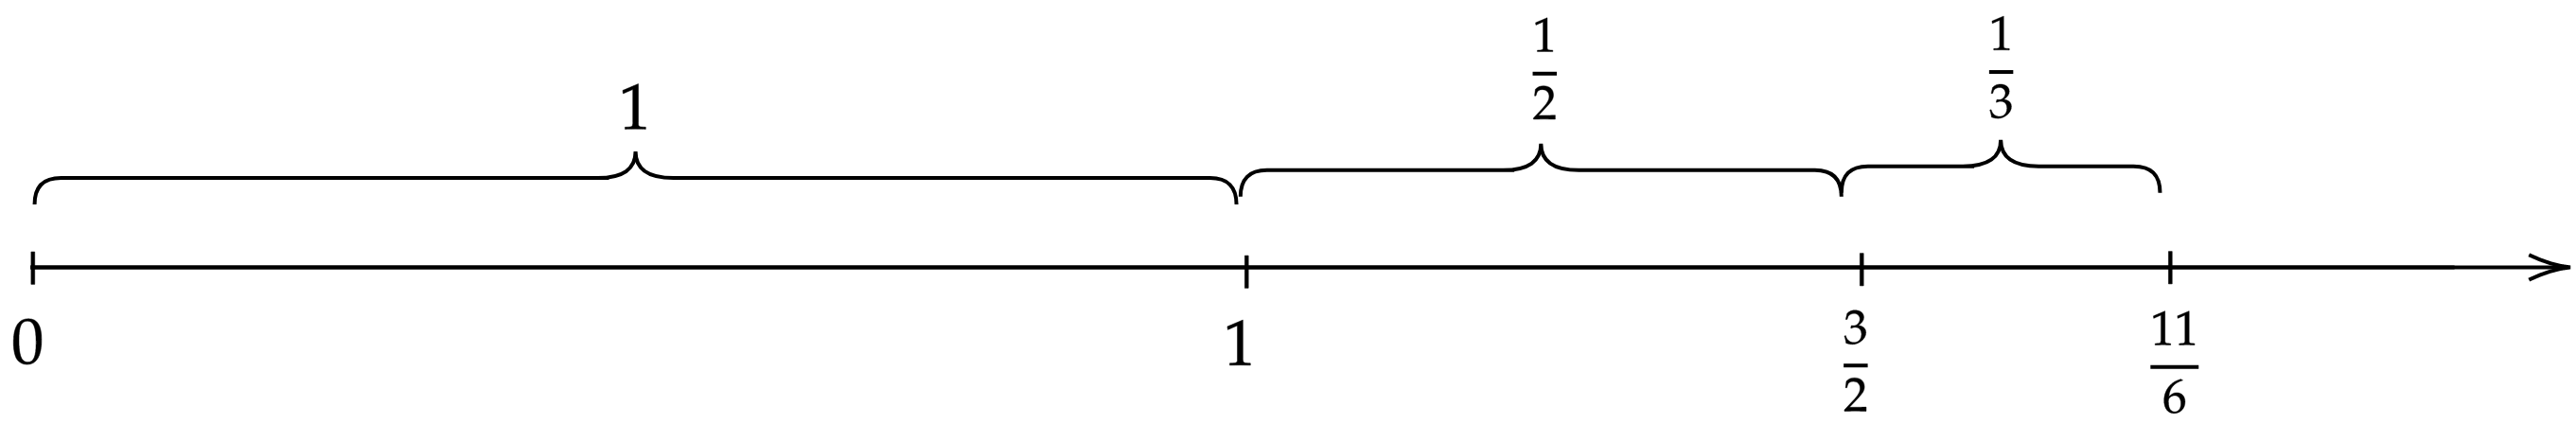
\includegraphics[width = 1\textwidth]{fig2.png}
    \caption{Геометрическая иллюстрация к суммированию ряда (\ref{eq:1}).}
    \label{fig:2}
\end{figure}
Поэтому кажется разумным положить, что существует некий предел, некое число $N$, которое сумма ряда точно не достигнет:
\begin{equation}\label{eq:7}
    1 + \dfrac{1}{2} + \dfrac13 + \dfrac14 + \dfrac15 + \ldots < N.
\end{equation}
Чтобы показать, что мы ошибаемся в данном предположении, рассмотрим такой ряд:
\begin{equation}\label{eq:9}
    \begin{split}
        &1 + \tfrac12 +\\
        &+ \tfrac14 + \tfrac14 +\\
        &+ \tfrac18+ \tfrac18+ \tfrac18+ \tfrac18 +\\
        &+ \tfrac1{16}+ \tfrac1{16}+ \tfrac1{16}+ \tfrac1{16} + \tfrac1{16}+ \tfrac1{16}+ \tfrac1{16}+ \tfrac1{16} + \ldots
    \end{split}
\end{equation}
Данный ряд составлен из слагаемых, которые представляют собой суммы $2^{n-1}$ подслагаемых, равных ${1}/{2^n}$ (например, сумма двух ${1}/{4}$), где $n$~\----~натуральное число. Тогда любая частичная сумма гармонического ряда будет больше  частичной суммы такого же количества элементов ряда (\ref{eq:9}) (если рассматривать лишь суммы, содержащие больше двух слагаемых). Действительно, сумма четырёх элементов ряда (\ref{eq:9}) будет равна $2$, частичная сумма четырёх элементов гармонического ряда равна $25/{2}$; сумма восьми элеметов ряда (\ref{eq:9}) равна $25/2$, в то время как сумма восьми элементов гармонического ряда даст ${761}/{280}$ и так далее.
\par
Сделаем одно важное замечание про ряд (\ref{eq:9}). Так как ряд разбивается на подсуммы, то каждую из них можно сразу просуммировать. Проделаем это:
\begin{equation}
    \begin{split}
        &1 = 1\\
        &\dfrac{1}{2} = \dfrac{1}{2}\\
        &\dfrac{1}{4} + \dfrac{1}{4} = \dfrac{1}{2}\\
        &\dfrac1{16}+ \dfrac1{16}+ \dfrac1{16}+ \dfrac1{16} + \dfrac1{16}+ \dfrac1{16}+ \dfrac1{16}+ \dfrac1{16} = \dfrac{1}{2} \quad \text{и так далее.}
    \end{split}
\end{equation}
Тогда исходный ряд (\ref{eq:9}) запишется:
\begin{equation}
    1 + \dfrac12 + \dfrac12 + \dfrac12 + \ldots
\end{equation}
Ясно, что сумма такого ряда не конечна. Она бесконечно велика. Такие ряды называют \emph{расходящимися} (более строгое определение будет дано ниже). Но если ряд (\ref{eq:9}), каждая частичная сумма которого меньше частичной суммы того же количесва членов гармонического ряда, расходится, то и гармонический ряд тоже расходится.
\subsection{Определения сходящихся и расходящихся рядов}
Дадим строгое математическое определение расходящегося ряда с неотрицательными слагаемыми. На языке кванторов оно запишется следующим образом.
\begin{definition}
Ряд с неотрицательными членами 
\begin{equation}\label{eq:12}
    \sum_{k=1}^\infty a_k, \quad a_k \ge 0
\end{equation}
называется расходящимся, если
\begin{equation}
    \forall N > 0 \quad \exists n: \quad a_1 + a_2 + \ldots + a_n > N.
\end{equation}
\end{definition}
То есть для любого сколь угодно большого положительного числа $N$ найдётся такое натуральное число $n$, что частичная сумма $n$ элементов ряда будет больше $N$. Иными словами сумма ряда больше любого действительного числа.
\par
Определение {сходящегося ряда с неотрицательными слагаемыми} с помощью кванторов записывается следующим образом.
\begin{definition}
Ряд с неотрицательными членами (\ref{eq:12}) называется сходящимя (или ограниченным), если 
\begin{equation}
    \exists N > 0: \quad \forall n \quad a_1 + a_2 + \ldots + a_n < N.
\end{equation}
\end{definition}
То есть существует такое положительное число $N$, что для любого натурального $n$ частичная сумма $n$ элементов ряда будет меньше $N$.
\section{Аксиома полноты}
\subsection{Ещё раз про расходящиеся и сходящиеся ряды}
Продолжаем рассматривать ряды с неотрицательными элементами. Запишем в общем виде такой ряд:
\begin{equation}\label{eq:15}
    a_0 + a_1 + a_2 + \ldots + a_n + \ldots
\end{equation}
Зададимся целью понять, можно ли придать данной бесконечной сумме некоторый смысл. То есть можно ли сопоставить данной бесконечной сумме число и утверждать, что это число равно данной бесконечной сумме?
\par
Мы уже поняли, что в случае расходимости такое число найти не удаётся. Действительно, в случае расходимости ряда положительных слагаемых для любого положительного числа $N$ хватит первых $n + 1$ слагаемых ряда (если нумеровать элементы начиная с индекса $0$), чтобы собрать из них сумму, большую $N$. Напомним, что на языке кванторов это запишется так:
\begin{equation}
    \forall N > 0 \quad \exists n: \quad a_0 + a_1 + \ldots + a_n > N.
\end{equation}
В случае расходимости ряда с неотрицательными слагаемыми его сумму символически обозначают за $+\infty$, где по определению $+\infty$~\----~"плюс бесконечность"{}~\----~символ, обозначающий некоторое число, которое больше любого действительного числа (это число не входит во множество действительных).
\par
Обратимся к противоположному случаю. Пускай существует такое положительное число $N$, что оно ограничевает ряд сверху. То есть для любого $n$ частичная сумма $n$ элементов будет меньше $N$. Запишем данное утверждение с помощью кванторов:
\begin{equation}\label{eq:17}
    \exists N>0: \quad \forall n \quad a_0+a_1+\ldots+a_n<N.
\end{equation}
Пускай факт ограниченности суммы ряда был установлен, можно ли из этого сделать вывод о том, что ряд сходится к какому\--то определённому значению, к какому\--то вещественному числу?
\subsection{Формулировка аксиомы полноты}
Ответ на данный вопрос связан с устройством действительных чисел и базируется на \emph{аксиоме полноты}. Проведём геометрическую аналогию суммирования ограниченного сверху ряда положительных элементов (см. рис. \ref{fig:3}). Видно, что ограниченный ряд должен куда\--то сходиться, что должна существовать некая точка, к которой стремятся частичные суммы.
\begin{figure}[ht]
    \centering
    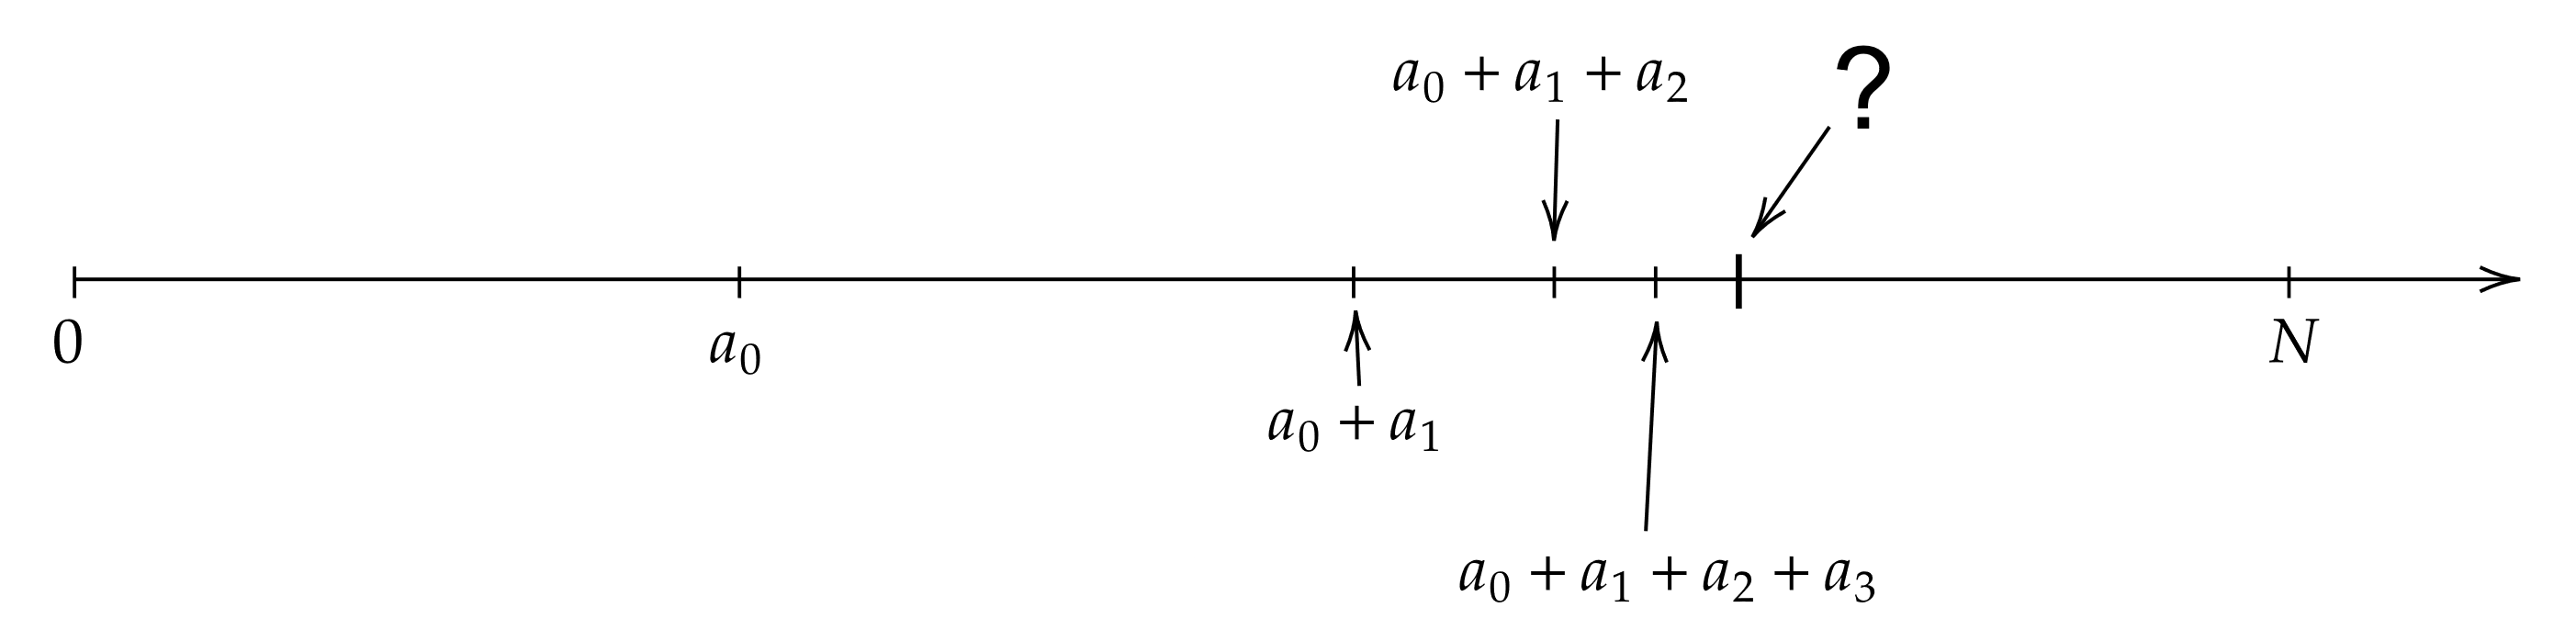
\includegraphics[width = 1\textwidth]{fig3.png}
    \caption{Геометрическая аналогия к процессу суммирования ряда положительных слагаемых, ограниченного сверху числом $N$. Вопросительный знак обозначает возможную сумму ряда.}
    \label{fig:3}
\end{figure}
Но везде ли на числовой прямой существуют числа? Вдруг предел частичных сумм попадёт в некий пробел, пустоту, то есть не будет лежать во множетсве действительных чисел? Ответ на данный вопрос может быть дан только аксиоматически. Пускай предел частичных сумм лежит на числовой прямой, то есть принадлежит ко множетсву действительных чисел. В этом и заключается аксиома полноты. Сформулируем её более строго. 
\begin{axiom}
{Ряд с неотрицательными элементами, который удовлетворяет свойству (\ref{eq:17}) (свойству ограниченности), сходится к конечному действительному значению}.
\end{axiom}
\subsection{Другая формулировка аксиомы полноты}
Существует множество эквивалентных формулировок данной аксиомы. Рассмотрим одну из них. Введём множество всех частичных сумм ряда положительных элементов (\ref{eq:15}):
\begin{equation}
    B = \qty{S_n = \sum_{i=0}^n a_i,\quad n\in \mathbb {N}}.
\end{equation}
Попробуем взять максимальный элемент множества $B$. Вообще говоря, это может не выйти. Вспоминим ряд (\ref{eq:2}). Мы договорились, что по определению его сумма равна $2$:
\begin{equation}
    1 + \dfrac{1}{2} + \dfrac14 + \dfrac18 + \dfrac{1}{16} + \ldots = 2.
\end{equation}
Для данного ряда множество $B$ предсавляло собой:
\begin{equation}
    \begin{split}
        B &= \qty{1,\dfrac{3}{2},\dfrac74,\dfrac{15}{8},\ldots}\\
        &=\qty{2-1,2-\dfrac{1}{2},2-\dfrac{1}{4},2-\dfrac{1}{8},\ldots}.
    \end{split}
\end{equation}
Видно, что с увеличением индекса элементов множества $B$ они сильнее сгущаются около $2$ (см. рис. \ref{fig:4}). То есть если взять сколь угодно малое $\varepsilon$ и рассмотреть интервал $\qty(2-\varepsilon,2)$, то в него попадут все точки множетсва $B$, за исключением некоторого конечного числа первых элементов.
\begin{figure}[ht]
    \centering
    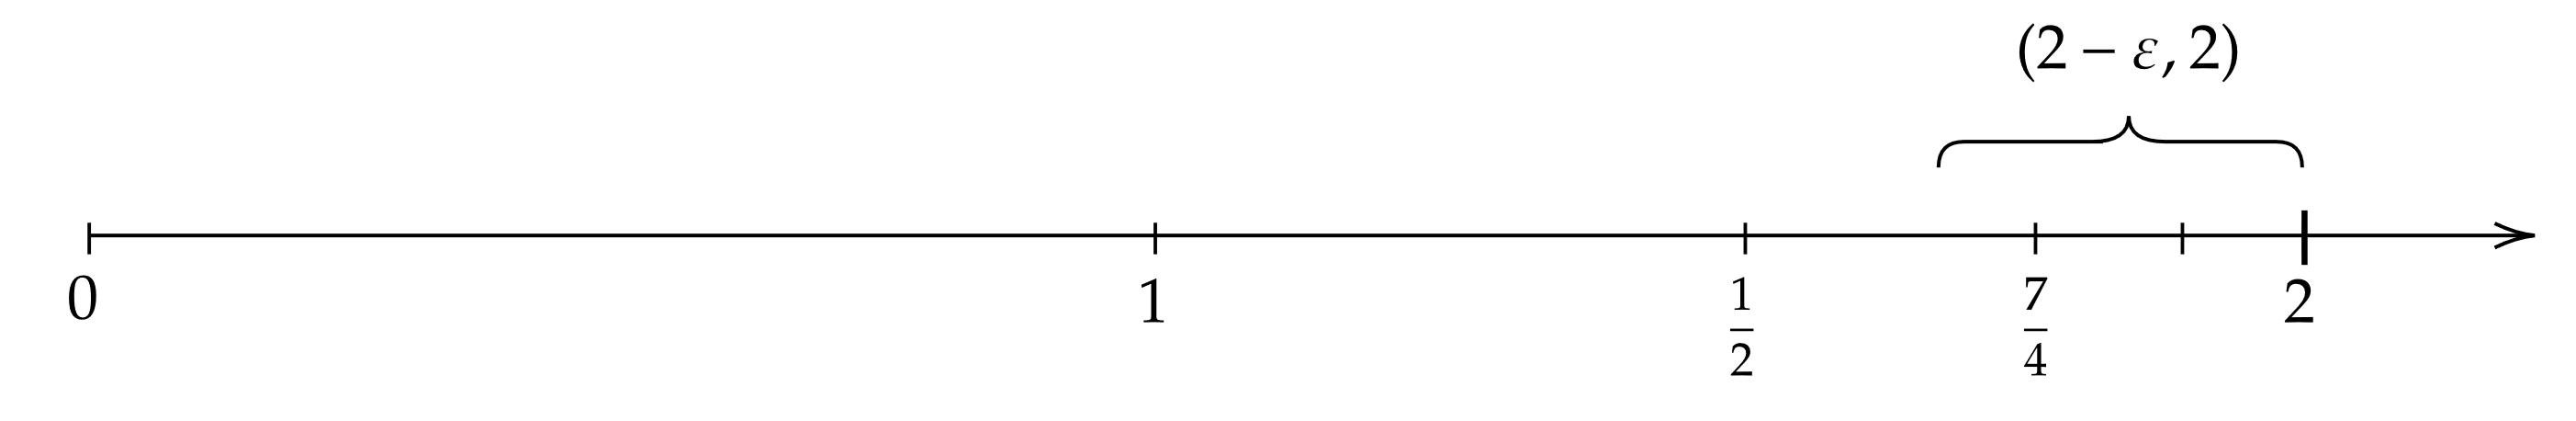
\includegraphics[width = 1\textwidth]{fig4.png}
    \caption{Геометрическая иллюстрация множества $B$ для ряда (\ref{eq:2}).}
    \label{fig:4}
\end{figure}
Ясно, что множество $B$ для ряда (\ref{eq:2}) не имеет максимального элемента, потому что для любого положительного действительного числа, меньшего $2$, найдётся элемент множества $B$, который больше данного числа, а любое число, большее либо равное $2$, находится вне множества $B$. С другой стороны число $2$~\----~наименьшее число, которое больше всех элементов множетсва $B$. На математическом языке данное замечание можно записать таким образом:
\begin{equation}
    \begin{split}
        &\forall x \in B \quad 2>x;\\
        &\forall M: \forall x \in B \quad x<M \Longrightarrow M \ge 2.
    \end{split}
\end{equation}
То есть сказано следующие. $2$ больше всех чисел из $B$, но меньше либо равно всех чисел, больших всех элементов из $B$.
\par
Введём некоторые новые концепции. Прежде всего определим множество $U\qty(B)$:
\begin{equation}
    U\qty(B) = \qty{M \in \mathbb{R}:\quad M \ge x \quad \forall x\in B}.
\end{equation}
Это множество действительных чисел, которые больше всех элементов множества $B$. Теперь определим понятие \emph{супремума множества}:
\begin{equation}
    \sup\qty(B) = \min U\qty(B).
\end{equation}
То есть мы берём множество всех чисел, которые больше элементов множества $B$, и минимум получившегося набора называем супремумом $B$.
\par
Можно заметить, что для множества $B$ ряда (\ref{eq:2}) множеством $U\qty(B)$ является луч [$2,+\infty$), тогда в нём существует минимум и он равен $2$. Выходит, что супремумом множества $B$ в этом случае по определению является число $2$.
\par
Возвращаемся к вопросу о существовании значения суммы ряда, составленного из положительных слагаемых (см. рис. \ref{fig:3}). Пускай мы откуда\--то знаем, что сумма ряда ограничена. Отсюда сразу следует, что множество $U\qty(B)$ не пусто (за множество $B$ обозначено множество частичных сумм рассматриваемого ряда). Значит, существует и минимум множества $U\qty(B)$, определённый нами, как супремум множества $B$. Тогда $\sup B$ в свою очередь по определению суммы ряда, состоящего из положительных элементов, является суммой рассматриваемого ряда:
\begin{equation}
    \sup B = a_0 + a_1 + a_2 + \ldots
\end{equation}
Таким образом, утверждением, равносильным аксиоме о полноте множества вещественных чисел, будет следующее утверждение. 
\begin{axiom}
{Множество $B$ для любого сходящегося ряда с неотрицательными элементами имеет вид бесконечного направо луча [$A,+\infty$), где $A$~\----~сумма ряда}.
\end{axiom}
\section{Сходимость ряда обратных квадратов}
\subsection{Доказательство сходимости ряда обратных квадратов}
Обратимся к следующему примеру: рассмотрим ряд
\begin{equation}\label{eq:25}
    1 + \dfrac{1}{4} + \dfrac{1}{9} + \ldots + \dfrac{1}{n^2} + \ldots
\end{equation}
Зададимся вопросом о сходимости данного ряда. Мы уже знаем, что очень похожий на него ряд, называемый гармоническим, относится к классу расходящихся рядов. Что же происходит с данным рядом? Для ответа на данный вопрос мы покажем, что данный ряд на самом деле является ограниченным (а, следовательно, и сходящимся). 
\par
Покажем, что сумма ряда (\ref{eq:25}) меньше $2$. Запишем ряд в виде:
\begin{equation}
    1 + \dfrac{1}{2\vdot 2} + \dfrac{1}{3\vdot 3} + \ldots + \dfrac{1}{n\vdot n} + \ldots
\end{equation}
Можно ограничить ряд (\ref{eq:25}) рядом, каждая частичная сумма которого не меньше соответствующей частичной суммы ряда (\ref{eq:25}). Данному свойству удовлетворяет ряд:
\begin{equation}\label{eq:26}
    1 + \dfrac{1}{1\vdot2} + \dfrac{1}{2\vdot3} + \ldots + \dfrac{1}{\qty(n-1)\vdot n} + \ldots
\end{equation}
Он и вправду больше ряда (\ref{eq:25}), ибо каждый его член, за исключением первого, больше соответствующего члена ряда (\ref{eq:25}).
Ряд (\ref{eq:26}) может быть переписан в следующем виде:
\begin{equation}
\begin{split}
        &1 + \dfrac{1}{1\vdot2} + \dfrac{1}{2\vdot3} + \ldots + \dfrac{1}{\qty(n-1)\vdot n} + \ldots =\\
    & = 1 + \qty(\dfrac{1}{1} - \dfrac{1}{2}) + \qty(\dfrac{1}{2}  - \dfrac{1}{3}) + \ldots +\qty(\dfrac{1}{n-1} - \dfrac{1}{n}) + \ldots
\end{split}
\end{equation}
Если теперь раскрыть скобки и провести сокращение подобных членов для частичной суммы первых $n$ членов ряда (\ref{eq:26}), то получим:
\begin{equation}
    \begin{split}
        1 + \dfrac{1}{1} - \cancel{\dfrac{1}{2}} + \cancel{\dfrac{1}{2}}  - \cancel{\dfrac{1}{3}} + \ldots +\cancel{\dfrac{1}{n-1}} - \dfrac{1}{n} = 2 - \dfrac{1}{n} < 2
    \end{split}
\end{equation}
То есть сумма первых $n$ членов ряда (\ref{eq:26}) всё ближе и ближе подходит к $2$ с увеличением $n$, но всегда остаётся меньше $2$. Ясно, что ряд (\ref{eq:26}) сходящийся. Мы можем даже утверждать, что сумма ряда (\ref{eq:26}) равна $2$, ведь $2$ является супремумом множества всех частичных сумм ряда (\ref{eq:26}).
\par
Теперь вспомним, что ряд (\ref{eq:25}) меньше ряда (\ref{eq:26}). Если больший из них ограничен, то и меньший обязан быть ограничен. Получается, что мы доказали, что ряд (\ref{eq:25}) меньше $2$:
\begin{equation}
    1 + \dfrac{1}{4} + \dfrac{1}{9} + \ldots + \dfrac{1}{n^2} + \ldots < 2.
\end{equation}
Великий математик Эйлер доказал, что сумма ряда (\ref{eq:25}) равна ${\pi^2}/{6}$.
\subsection{Геометрическая интерпритация рядов}
Рассмотренные выше ряды (\ref{eq:25}) и (\ref{eq:26}) имеют простую геометрическую интерпритацию. Сперва обратимся к геометрической иллюстрации ряда (\ref{eq:26}). Будем рисовать прямоугольники со сторонами, как при разбиении на множители типа $a_n = {1}/\qty{\qty(n-1)n}$ (то есть со сторонами ${1}/\qty(n-1)$ и ${1}/{n}$). По идее они должны умещаться в прямоугольник со сторонами $1$ и $2$. Вопрос о том, возможно ли разместить такие прямоугольники в прямоугольнике с площадью $2$, остаётся открытым и по сей день \cite{1,2,3}, поэтому ограничемся размещением лишь нескольких первых прямоугольников (см. рис. \ref{fig:5}).
\begin{figure}[ht]
    \centering
    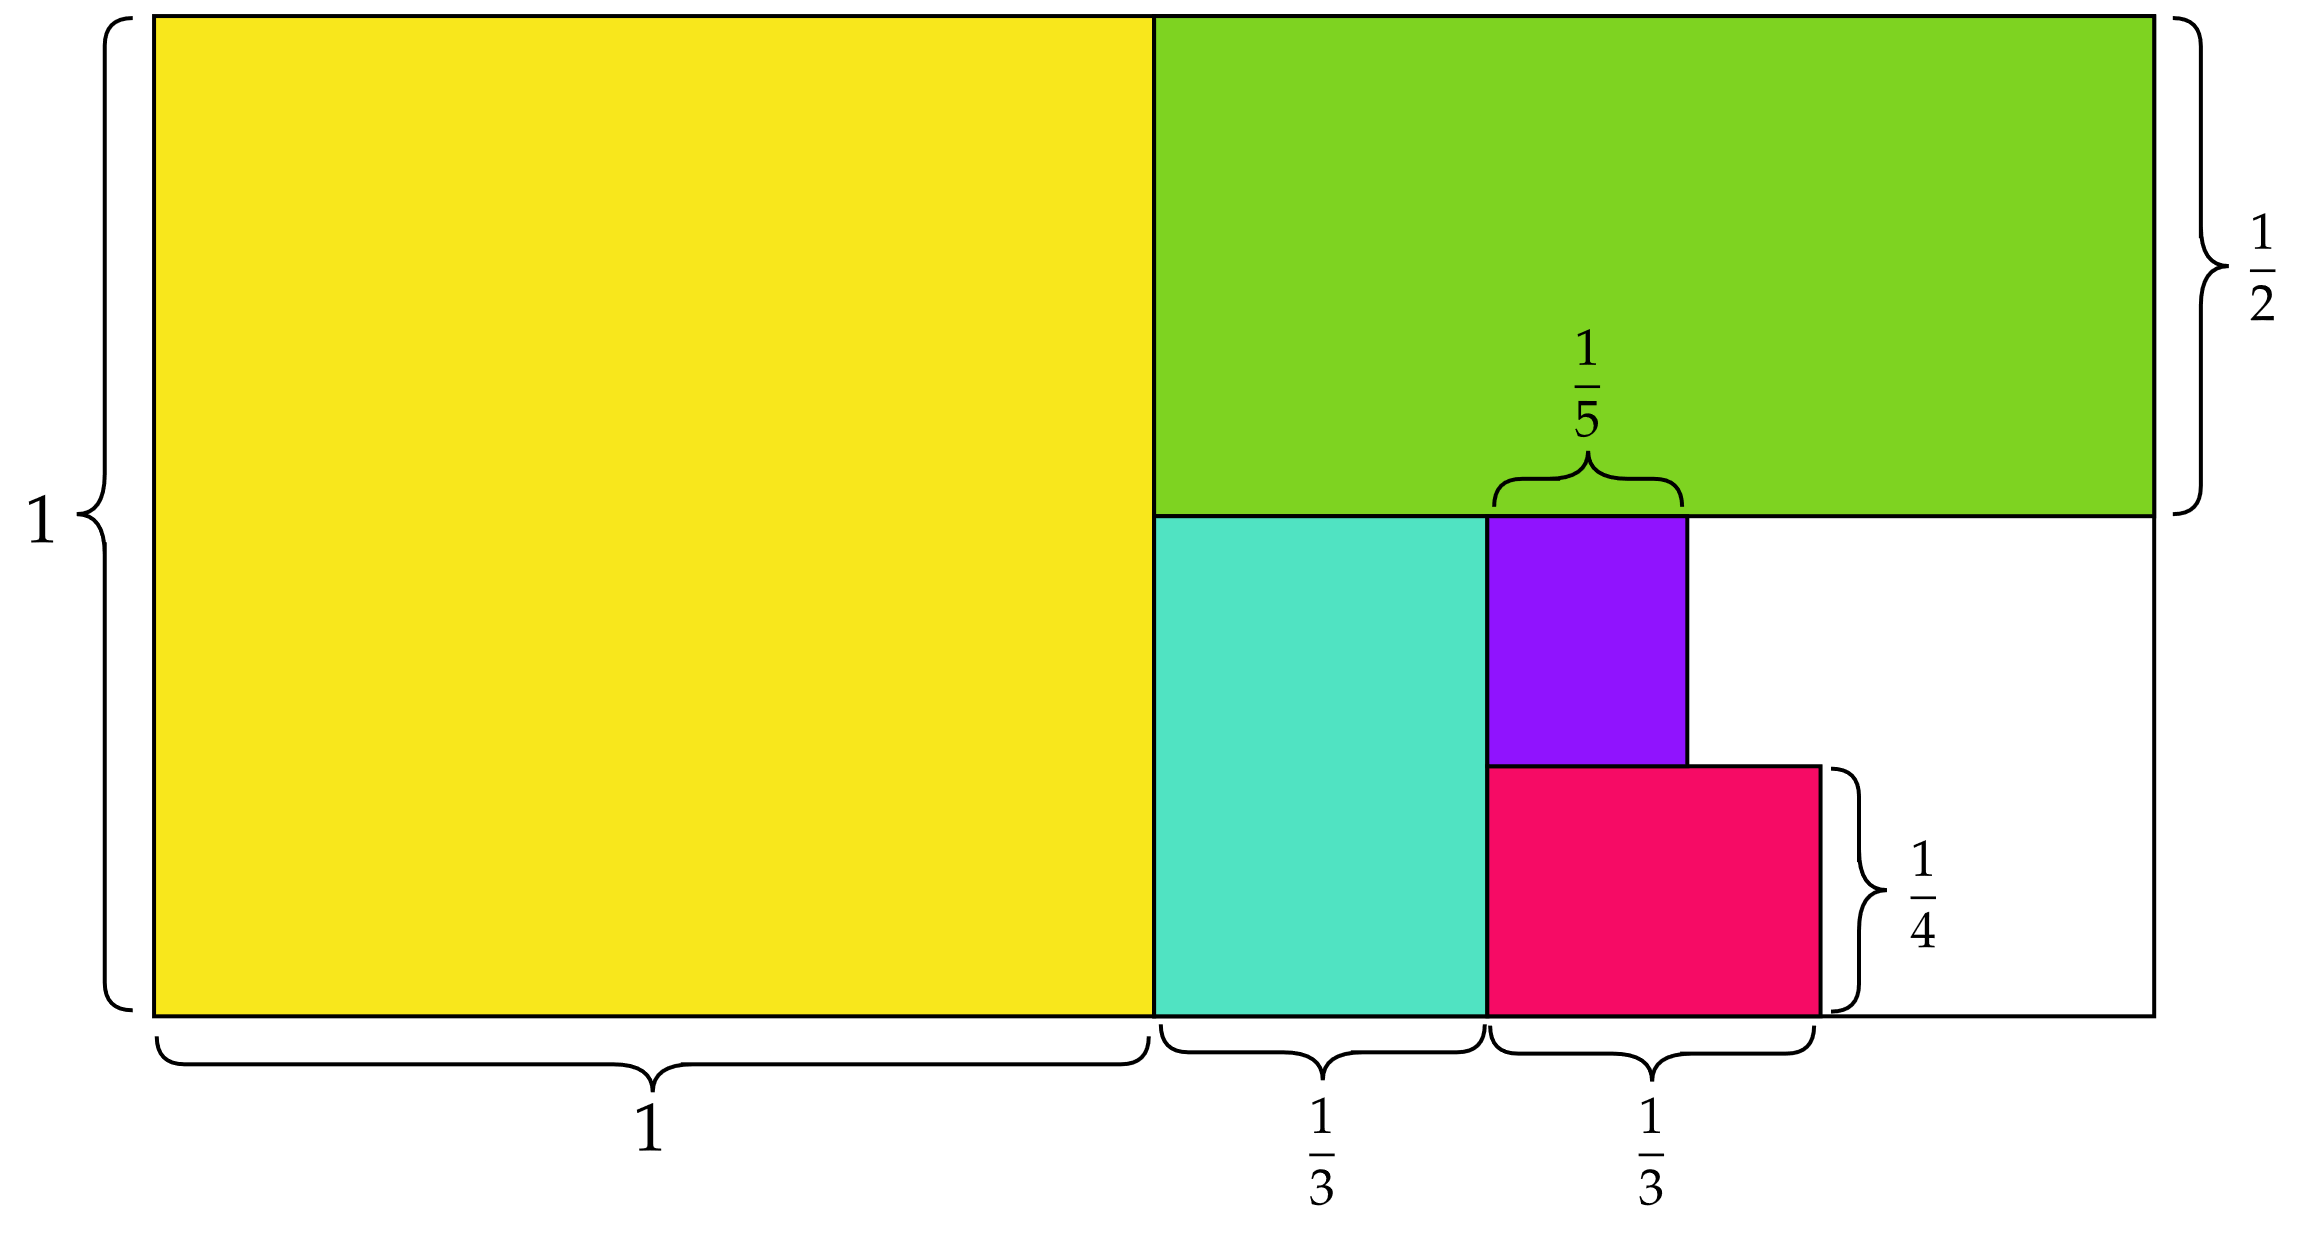
\includegraphics[width = 1\textwidth]{fig5.png}
    \caption{Геометрическая интерпритация ряда ${1}/\qty{\qty(n-1)n}$.}
    \label{fig:5}
\end{figure}
\par
Нужно помнить, что если невозможно разместить прямоугольники таким образом, чтобы они не перекывались, в прямоугольнике со сторонами $1$ и $2$, то отсюда вовсе не следует расходимость ряда. Ряд как раз сходится, а вот можно ли так разместить прямоугольники~\----~пока неизвестно.
\par
Что же касается ряда (\ref{eq:25}), то для него возможна аналогичная иллюстрация. Стартуем с прямоугольника со сторонами $1$ и $2$, разделяем его на квадраты со сторонами $1$, левый квандрат соответствует первому члену ряда, правый отдаётся под размещение всех остальных прямоугольников по приведённому ниже правилу. Делим правый квадрат пополам по горизонтали, верхнюю часть делим пополам по вертикали. Левой части соответсвует элемент ряда ${1}/{4}$, правой~\----~${1}/{9}$ (см. рис. \ref{fig:6}). Повторяем данную процедуру: делим нижний прямоугольник со сторонами $1$ и ${1}/{2}$ пополам по горизонтали, верхний получившийся прямоугольник делим на четыре части по вертикали, в каждую из них вписываем прямоугольник, отвечающий члену ряда, и так далее.
\begin{figure}[ht]
    \centering
    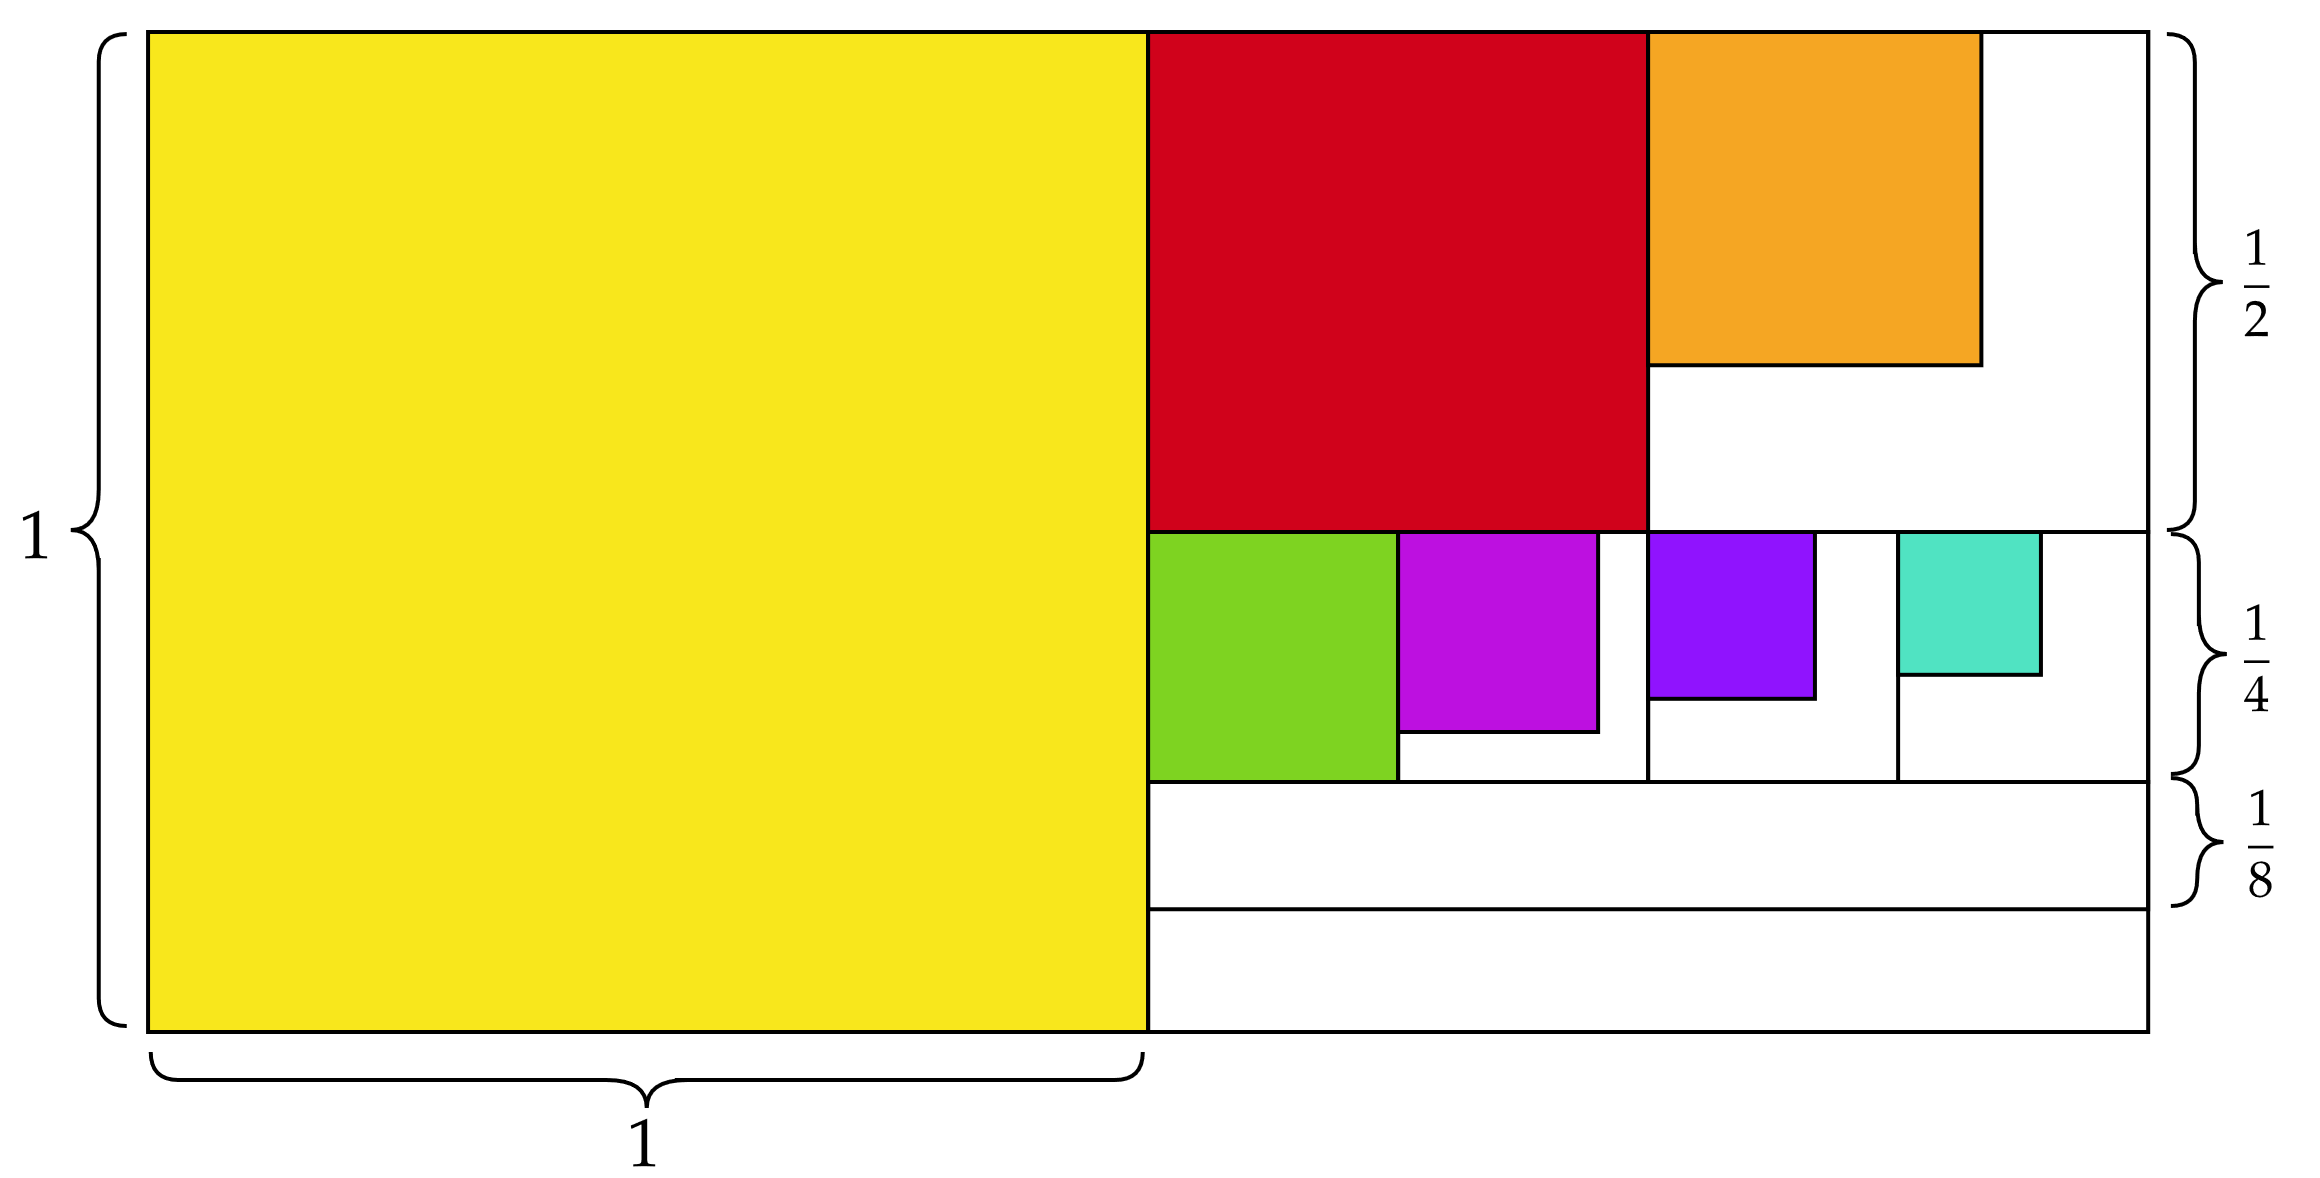
\includegraphics[width = 1\textwidth]{fig6.png}
    \caption{Геометрическая интерпритация ряда ${1}/{n^2}$.}
    \label{fig:6}
\end{figure}
\par
Видно, что площадь квадратов, отвечающих элементам ряда, не покрывает всей площади исходного прямоугольника, это отражает тот факт, что сумма ряда (\ref{eq:25}) меньше двух.




\subsection{Выводы}
Пускай имеются два ряда с неотрицательными членами:
\begin{eqnarray}
a_0 + a_1 + a_2 + \ldots,
\label{eq:32_a}
\\
b_0 + b_1 + b_2 + \ldots, \label{eq:32_b}
\end{eqnarray}
а их элементы удовлетворяют условию
\begin{equation}\label{eq:32}
    \forall n \in \mathbb{N} \Longrightarrow a_n \ge b_n \ge 0.
\end{equation}
Тогда можно сформулировать два достаточных условия: досаточное условие сходимости и достаточное условие расходимости. 
\par
Достаточное условие расходимости формулируется следующим образом.
\begin{theorem}
Если выполняется \eqref{eq:32},
то из расходимости ряда (\ref{eq:32_b}) следует расходимость ряда (\ref{eq:32_a}).
\end{theorem}
Достаточное условие сходимости формулируется схожим образом.
\begin{theorem}
Если выполняется (\ref{eq:32}), то из сходимости ряда (\ref{eq:32_a}) следует сходимость ряда (\ref{eq:32_b}).
\end{theorem}
\section{Перегруппировка слагаемых}
При суммировании ряда бывает полезным следующий приём. Слагаемые можно разбить в суммы подслагаемых, далее можно их перегруппировать на другие, более удобные суммы. Мы уже пользовались данным методом, когда вычисляли сумму ряда 
\begin{equation}
    \sum_{n=1}^\infty \dfrac{1}{n\qty(n+1)}.
\end{equation}
\par
Существует важное замечание к данному методу. Перед его применением важно доказать, что ряд сходится, ведь данный метод может дать некий ответ, не имеющий ничего общего с действительностью, в случае расходящегося ряда. Продемонстрируем это на примере. Рассмотрим ряд
\begin{equation}
    \sum_{n=1}^\infty a_n, \text{ где } a_n = \dfrac{1}{\sqrt{n+1} + \sqrt{n}}.
\end{equation}
Просуммируем ряд следующим способом~\----~умножим и поделим каждый член ряда на скобку $\qty(\sqrt{n+1} - \sqrt{n})$. Получим тогда выражение для общего члена ряда:
\begin{equation}
    a_n = \dfrac{1}{\sqrt{n+1} + \sqrt{n}} = \sqrt{n+1} - \sqrt{n}.
\end{equation}
Далее возникает желание просуммировать данный ряд следующим образом:
\begin{equation}
    a_1+a_2+a_3+\ldots = \cancel{\sqrt{2}} - \sqrt{1} + \cancel{\sqrt{3}} - \cancel{\sqrt{2}} +\sqrt{4} - \cancel{\sqrt{3}} + \ldots
\end{equation}
Если сократить подобные слагаемые, то получится ответ равный $-1$. Это противоречит тому факту, что ряд мы суммировали с неотрицательными членами, следовательно, никак не могли получить отрицательный результат. Дело тут в том, что исходный ряд является расходящимся. Действительно, рассмотрим частичные суммы
\begin{equation}
    S_n = \sqrt{2} - \sqrt{1} + \sqrt{3} - \sqrt{2} + \ldots + \sqrt{n+1} - \sqrt{n} = \sqrt{n+1} -1.
\end{equation}
Видно, что частичные суммы при увеличении $n$ неограниченно растут до $+\infty$. Ряд расходится. Поэтому метод перегруппировки слагаемых ряда даёт неверный ответ.
\section{Интегральный признак}
\subsection{Теория}
Рассмотрим один из способов проверки сходимости рядов с положительными членами, который называется \emph{интегральный признак}. Данный признак сходимости основан на понятии интеграла, что будет дано на более поздних лекциях.
\par
Итак, рассматриваем ряд с неотрицательными членами $\sum_{n=1}^\infty a_n$. Пускай члены ряда убывают в нестрогом смысле, то есть
\begin{equation}
    a_{n} \ge a_{n+1} \ge 0, \quad n\in \mathbb{N}.
\end{equation}
Будем обозначать через $S_n$ $n$\--ую частичную сумму ряда:
\begin{equation}
    S_n = \sum\limits_{i=1}^n a_i.
\end{equation}
Тогда сумма ряда $S$, если она, конечно, существует, будет являться пределом последовательности частичных сумм или точной верхней гранью последовательности частичных сумм. Ответ на вопрос о сходимости ряда зависит от того, ограничена ли последовательность частичных сумм или нет. Если ограничена, то ряд сходится, если нет, то ряд расходится.
\par
Чтобы проверить ограниченность последовательности частичных сумм рассмотрим следующее. Построим график последовательности членов рассматриваемого ряда (см. рис. \ref{fig:7}).
\begin{figure}[ht]
    \centering
    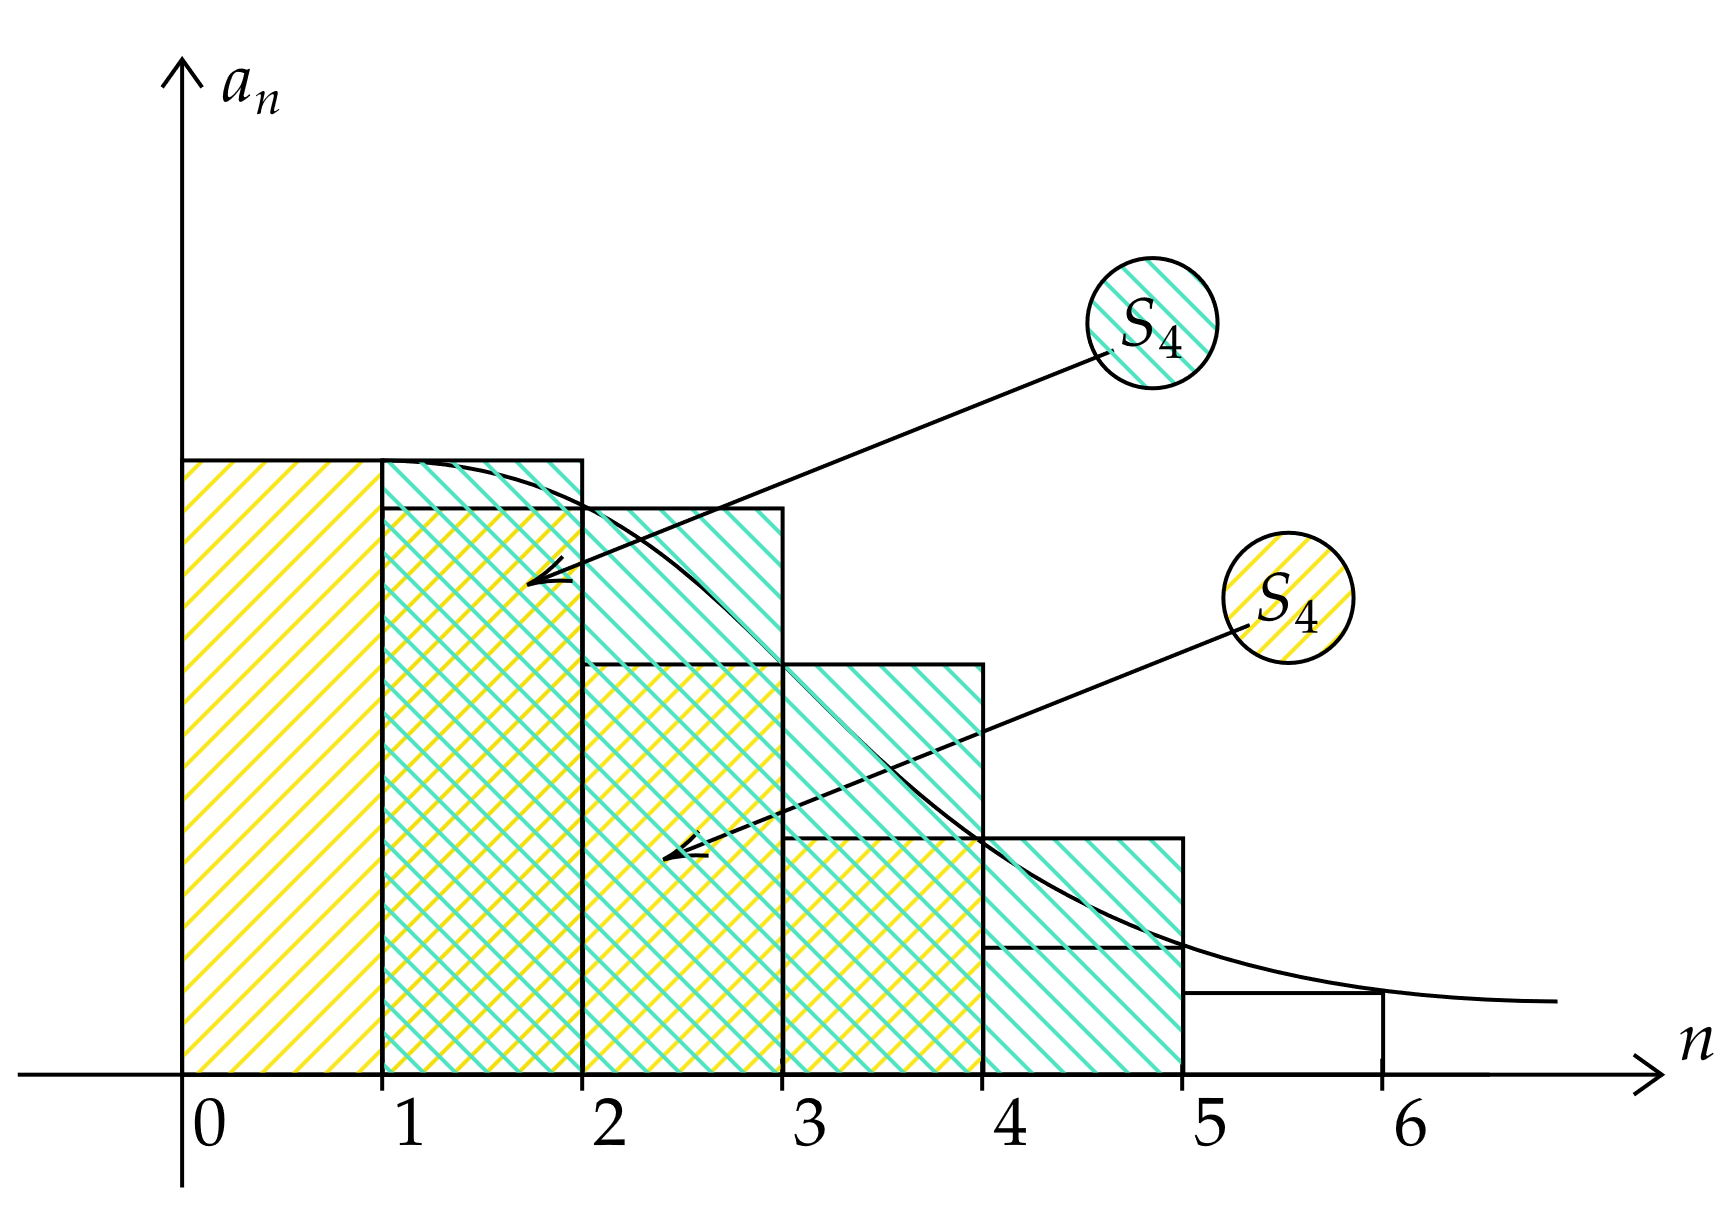
\includegraphics[width = 1\textwidth]{fig7.png}
    \caption{График слагаемых ряда с неотрицательными членами, которые убывают в нестрогом смысле.Жёлтой штриховкой закрашена частичная сумма $S_4$. Она же, сдвинутая на единицу вдоль оси $n$, закрашена голубой штриховкой.}
    \label{fig:7}
\end{figure}
На данном графике закрашены штриховкой частичная сумма $S_4$ и она же, но сдвинутая на единицу вдоль оси $n$. Проведём через точки членов ряда непрерывную убывающую кривую. Назовём соответствующую ей функцию $f\qty(x)$. Теперь попробуем оценить частичную сумму ряда с помощью интеграла от данной функции. Обозначим интеграл следующим образом:
\begin{equation}
    s\qty(x) = \int\limits_1^x f\qty(t) \dd t.
\end{equation}
Его смысл заключается в том, что он равен площади криволинейной фигуры, образуемой под графиком функции $f\qty(x)$ от $1$ до $x$. Из графика видно, что $s\qty(5) < S_4$ (см. желтую штриховку). Если же брать синюю штриховку, то можно заметить, что $S_4 < s\qty(4) + a_1$. Тогда получаем, что:
\begin{equation}
    s\qty(5) < S_4 <  s\qty(4) + a_1.
\end{equation}
Очевидно обобщение на любую частичную сумму:
\begin{equation}\label{eq:44}
    s\qty(n+1) < S_n < s\qty(n) + a_1.
\end{equation}
Из этого неравенства вытекает интегральный признак сходимости.
\begin{theorem}
Если $s\qty(n+1)$ расходится, то и $S_n$ расходится; если же $s\qty(n)$ сходится, то и $S_n$ сходится. Более того, можно оценить сумму ряда с помощью двойного неравенства (\ref{eq:44}). Если сумма ряда существует, то можно проинтегрировать функцию $f\qty(x)$ до бесконечности и получить такую оценку:
\begin{equation}
    s < S < s + a_1.
\end{equation}
\end{theorem}
Данный метод очень удобен в случае, когда $f\qty(x)$ выражается через явные функции, тогда просто легче вычислить от неё интеграл, чем вычислять сумму ряда.
\subsection{Примеры}
Рассмотрим ещё несколько характерных примеров. Во\--первых, вновь посмотрим на гармонический ряд. Из предыдущих секций известно, что данный ряд расходится. Напомним, что в данном ряду элемент имеет такой вид:
\begin{equation}
    a_n = \dfrac{1}{n}.
\end{equation}
Тогда функция, проходящая через все элементы даннного ряда будет иметь схожий вид:
\begin{equation}
    f\qty(x) = \dfrac{1}{x}.
\end{equation}
Интегрируя её, получаем функцию для суммы:
\begin{equation}
    s\qty(x) = \ln{x}.
\end{equation}
Имеем логарифм (см. рис. \ref{fig:8}). Он неограниченно, хоть и очень медленно, растёт до бесконечности. Значит, ряд расходится. Что и требовалось показать.
\begin{figure}[hbt]
    \centering
    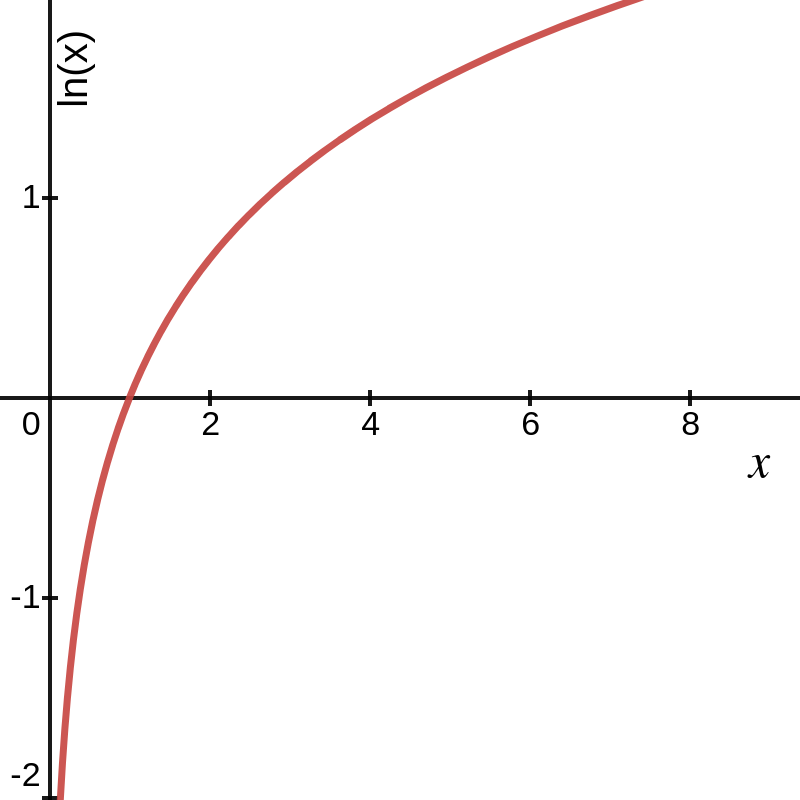
\includegraphics[scale = 0.5]{fig8.png}
    \caption{График натурального логарифма $f\qty(x) = \ln{x}$.}
    \label{fig:8}
\end{figure}
\par
В качестве второго примера возьмём ряд с членами, вида:
\begin{equation}
    a_n = \dfrac{1}{n^2}.
\end{equation}
Функция будет иметь вид:
\begin{equation}
    f\qty(x) = \dfrac{1}{x^2}.
\end{equation}
Берём интеграл\footnote{Тут пользуемся тем фактом, что первообразная от степенной функции $x^n$ есть функция $F(x)=nx^{n+1}.$ Кроме того, используем формулу Ньютона\--Лейбница, известную со школы:
$ \int_a^b f\qty(x) = \eval{F\qty(x)}_a^b$.} и получаем площадь под данной функцией:
\begin{equation}
    s\qty(x) = 1 - \dfrac{1}{x}.
\end{equation}
Видно, что площадь под графиком $f\qty(x)$ при стремлении правой границы к бесконечности (стремлении $x$ к бесконечности) стремится к $1$ (см. рис. \ref{fig:9}). Значит, ряд сходится, как и было показано ранее. 
\begin{figure}[hbt]
    \centering
    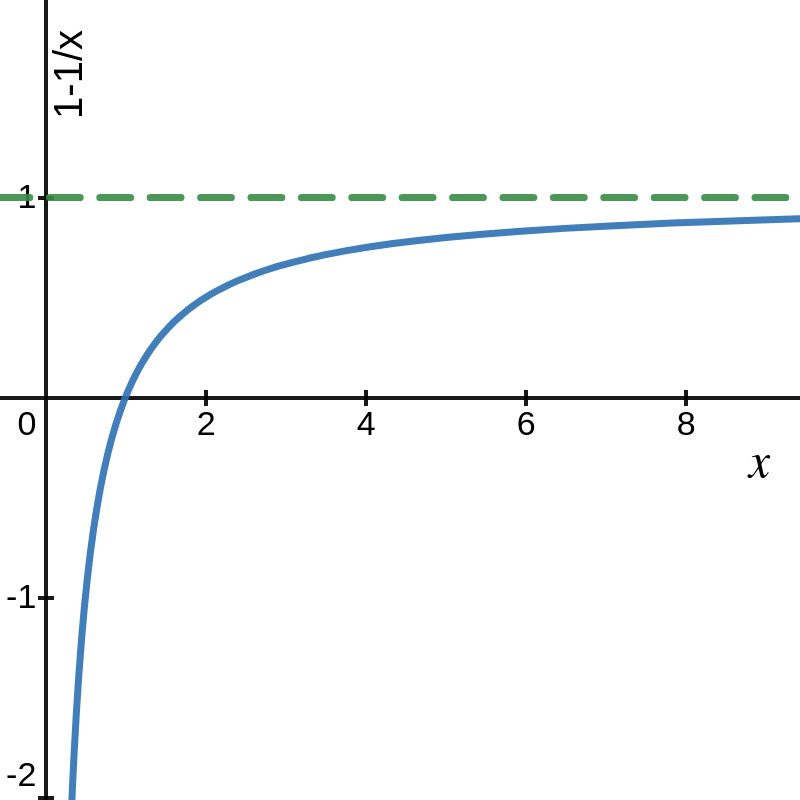
\includegraphics[scale = 0.5]{fig9.png}
    \caption{График функции $f\qty(x) = 1 - 1/x$. Видно, что она стремится к $1$ при росте $x$.}
    \label{fig:9}
\end{figure}
Оценим с помощью полученного двойного неравентства сумму данного ряда:
\begin{equation}
    1 < S < 1 + \dfrac{1}{1} = 2.
\end{equation}
Заметим, что известна точная сумма рассматриваемого ряда:
\begin{equation}
    S = \dfrac{\pi^2}{6} \approx 1.64.
\end{equation}
\section{Признаки Даламбера и Коши}
\subsection{Число Эйлера}
Продолжаем рассматривать признаки сходимости рядов с неотрицательными членами. Не всегда интегральный признак сходимости рядов может быть применён. Например, рассмотрим ряд, суммой которого является число Эйлера $e$:
\begin{equation}
    e = \sum\limits_{n=0}^\infty \dfrac{1}{n!},\text{ где } n! = \prod\limits_{k=1}^n k\text{ и }0! = 1.
\end{equation}
\begin{definition}
Число Эйлера $e$ определяется именно как сумма ряда
\begin{equation}
    \sum\limits_{n=0}^\infty \dfrac{1}{n!} = e.
\end{equation}
\end{definition}

\subsection{Признак сходимости Даламбера}
Зададимся вопросом о том, как доказать сходимость данного ряда. Существует много способов доказательства сходимости. Один из них подразумевает оценку общего члена ряда сверху членом геометрической прогрессии. Геометрическая прогрессия выбрана для рассмотрения не просто так. Дело в том, что ряд с членами в виде элементов геометрической прогрессии может быть легко просуммирован. Действительно, для геометрической прогрессии со знаменателем $0 \le q < 1$ можно легко вывести формулу\footnote{Мы уже знаем, что сумма ряда~\----~предел последовательности частичных сумм. Тогда рассмотрим частичную сумму геометрической прогресии, пользуясь школьными знаниями:
$$\sum_{n=0}^k q^n = \dfrac{1-q^k}{1-q}.$$
Стремим $k$ к бесконечности и получаем:
$$\lim_{k\rightarrow\infty} \dfrac{1-q^k}{1-q} = \dfrac{1}{1-q}.$$}:
\begin{equation}
    \sum\limits_{n=0}^\infty q^n = \dfrac{1}{1-q}.
\end{equation}
\par
Сформулируем признак сходимости Даламбера:
\begin{theorem}
    Если выполняется следующее требование:
    \begin{equation}
        \exists N: \forall n \ge N \Longrightarrow \dfrac{a_{n+1}}{a_{n}} \le q,
    \end{equation}
    где $0 \le q < 1$, то ряд сходится. Данный подход позволяет также оценить сумму ряда сверху:
    \begin{equation}
        S < S_{N-1} + \dfrac{a_N}{1-q}.
    \end{equation}
\end{theorem}
\begin{proof}
Пускай верно, что 
\begin{equation}
        \exists N: \forall n \ge N \Longrightarrow \dfrac{a_{n+1}}{a_{n}} \le q,
\end{equation}
где $0 \le q < 1$. Тогда можно записать следующую цепь неравенств:
\begin{equation}
    \dfrac{a_{N+1}}{a_N} \le q,\quad \dfrac{a_{N+2}}{a_{N+1}} \le q,\quad \ldots,\quad \dfrac{a_{N+k+1}}{a_{N+k}} \le q, \ldots
\end{equation}
Перемножаем первые $k$ данный неравенств. Получаем
\begin{equation}
    \dfrac{a_{N+1}}{a_{N}}\vdot \dfrac{a_{N+2}}{a_{N+1}}\vdot\ldots\vdot \dfrac{a_{N+k+1}}{a_{N+k}} = \dfrac{a_{N+k+1}}{a_N} \le q^k.
\end{equation}
Откуда имеем следующее:
\begin{equation}
    {a_{N+k+1}} \le {a_N} \vdot q^k,\quad k \ge 0.
\end{equation}
Мы получили, что ряд ограничен сверху бесконечной суммой элементов геометрической прогрессии:
\begin{equation}\label{eq:63}
    \sum_{k=0}^{\infty} {a_{N+k+1}} \le a_N \sum_{k=0}^{\infty} q^k.
\end{equation}
Ряд из элементов геометрической прогрессии сходится, как мы уже знаем, поэтому сходмость ряда 
\begin{equation}
    \sum_{k=0}^{\infty} {a_{N+k+1}}
\end{equation}
доказана. Что же касается исходного ряда, то первые $N-1$ члены не влияют на его сходимость, они лишь дадут какую\--то конечную добавку к сумме ряда. Получается, что и сходимость исходного ряда доказана.
\par
Обратимся к оценке суммы ряда. Для этого перепишем исходный ряд в виде:
\begin{equation}
    \sum_{n=0}^{\infty}a_n = \sum_{n=0}^{N-1}a_n+\sum_{k=0}^{\infty} {a_{N+k+1}}.
\end{equation}
Далее оцениваем второе слагаемое согласно (\ref{eq:63}) и считаем сумму ряда с элементами, образующими геометрическую прогрессию:
\begin{equation}
    \sum_{n=0}^{\infty}a_n \le \sum_{n=0}^{N-1}a_n+a_N \sum_{k=0}^{\infty} q^k = S_{N-1} + \dfrac{a_N}{1-q}.
\end{equation}
Теорема доказана.
\end{proof}
Рассмотрим ряд 
\begin{equation}
    \sum_{n=0}^\infty \dfrac{1}{n!}.
\end{equation}
По признаку Даламбера ряд сходится, ибо начиная с $n=1$ выполняется требование признака Даламбера:
\begin{equation}
    \dfrac{a_{n+1}}{a_n} = \dfrac{1}{n+1} \le \dfrac{1}{2}.
\end{equation}
То есть $q = {1}/{2}$. Кроме доказательства сходимости данный признак позволяет оценить сумму рассматриваемого ряда. Для начала положим $N = 1$. Тогда ${a_2}/{a_1} = {1}/{2}$ и сумма оценивается следующим образом:
\begin{equation}
    S \ge 1 + \dfrac{1}{1-\dfrac{1}{2}} = 3.
\end{equation}
Это достаточно грубая оценка числа $e$. Более хорошую оценку можно получить при рассмотрении больших $N$. Например, при $N = 2$ получаем $q = {1}/{3}$, тогда:
\begin{equation}
    S \ge 2 + \dfrac{\dfrac{1}{2}}{1 - \dfrac{1}{3}} = 2.75.
\end{equation}
Аналогично при $N = 3$ получаем $S \ge {49}/{18} = 2.7\qty(2)$. Первые же знаки десятичной записи числа Эйлера выглядят следующим образом:
\begin{equation}
    e = 2.71828\ldots
\end{equation}
\subsection{Признак сходимости Коши}
Существует и другой признак сходимости рядов, похожий по принципу действия на признак Даламбера~\----~признак Коши. Его формулировка выглядит так.
\begin{theorem}
    Если верно, что
    \begin{equation}
        \exists N:\forall n\ge N \Longrightarrow \sqrt[n]{a_n}\le q,
    \end{equation}
    где $0\le q < 1,$ то ряд сходится.
\end{theorem}
Можно с помощью признака Коши \cite{4} получить и оценку на сумму вышерассмотренного ряда, правда они получатся более грубыми, чем оценки, полученные с помощью признака Даламбера.

\medskip
\begin{thebibliography}{9}
\bibitem{1}
Bálint V., \textit{A Packing Problem and Geometrical Series}, Annals of Discrete Mathematics, Volume 51, Pages 17-21, \url{https://doi.org/10.1016/S0167-5060(08)70600-9} (1992)
\bibitem{2}
Jennings D., \textit{On packing unequal rectangles in the unit square}, Journal of Combinatorial Theory, Series A, Volume 68, Issue 2, Pages 465-469, \url{https://doi.org/10.1016/0097-3165(94)90116-3} (1994)
\bibitem{3}
Brass P., Moser W.O.J., and Pach J., Research Problems in Discrete Geometry, Springer New York, \url{https://doi.org/10.1007/0-387-29929-7} (2006)
\bibitem{4}
Пискунов Н. С., \textit{Дифференциальное и интегральное исчисления для втузов}, т. 2: Учебное пособие для втузов.—13-е изд.— М.: Наука, Главная редакция физико-математической литературы, 256 \--- 257 c, (1985)
\end{thebibliography}

\end{document}
